\documentclass[12pt,a4paper,openright,twoside]{book}
\usepackage[utf8]{inputenc}
\usepackage{disi-thesis}
\usepackage{code-lstlistings}
\usepackage{notes}
\usepackage{shortcuts}
\usepackage{acronym}
\usepackage{cleveref}

\acrodef{PC}{Personal Computer}
\acrodef{VNC}{Virtual Network Computing}
\acrodef{RDP}{Remote Desktop Protocol}
\acrodef{TPDU}{Transport Protocol Data Units}
\acrodef{PDU}{Protocol Data Units}
\acrodef{SVC}{Static Virtual Channels}
\acrodef{DCV}{Dynamic Virtual Channels}


\school{\unibo}
\programme{Corso di Laurea Triennale in Ingegneria e Scienze Informatiche}
\title{Evoluzione delle Tecnologie di Desktop Remoto}
\author{Matteo Susca}
\date{\today}
\subject{Reti di Telecomunicazioni}
\supervisor{Prof. Franco Callegati}
\session{I}
\academicyear{2023-2024}

% Definition of acronyms
\acrodef{IoT}{Internet of Thing}
\acrodef{vm}[VM]{Virtual Machine}


\mainlinespacing{1.241} % line spacing in mainmatter, comment to default (1)

\begin{document}

\frontmatter\frontispiece

\begin{abstract}	
Max 2000 characters, strict.
\end{abstract}

\begin{dedication} % this is optional
Optional. Max a few lines.
\end{dedication}

%----------------------------------------------------------------------------------------
\tableofcontents   
% \listoffigures     % (optional) comment if empty
% \lstlistoflistings % (optional) comment if empty
%----------------------------------------------------------------------------------------

\mainmatter

%----------------------------------------------------------------------------------------
\chapter{Introduzione}
\label{chap:introduction}

Al giorno d'oggi, è sempre più comune incontrare realtà lavorative che offrono la possibilità di lavorare da remoto.
%
La possibilità di connettersi ad un computer aziendale da qualsiasi dispositivo connesso a internet comporta numerosi e innegabili vantaggi,
come l'accesso diretto alla rete aziendale,
l'utilizzo di hardware specifico per alcune attività senza doverlo trasportare fisicamente,
e la flessibilità di lavorare da casa o in mobilità.
%
Tutto questo è reso possibile dalle tecnologie di desktop remoto, che permettono di controllare un computer da un altro dispositivo, ovunque esso si trovi, come se ci si trovasse fisicamente davanti ad esso.

Anche nell'industria videoludica le tecnologie di desktop remoto ricoprono un ruolo importante.
%
Il cloud gaming,
ad esempio, è un servizio che permette di giocare a videogiochi in streaming,
sfruttando la potenza di calcolo di un server remoto.
%
Il colosso tecnologico NVIDIA,
uno dei principali attori in questo settore,
ha dimostrato fin dal 2013 con il servizio NVIDIA GRID di essere in grado di offrire un'esperienza di gioco fluida e di alta qualità,
grazie all'utilizzo di tecnologie di desktop remoto.
%
Ora il servizio è stato ribattezzato GeForce NOW e offre la possibilità di giocare a numerosi titoli di successo,
anche su dispositivi mobili.
%
Anche altre aziende come Google,
Microsoft e Amazon stanno investendo in questo settore,
con servizi come Google Stadia (attualmente chiuso),
Xbox Cloud Gaming e Amazon Luna.

L'assistenza remota è un altro campo in cui le tecnologie di desktop remoto hanno avuto un impatto positivo.
%
I tecnici possono ora accedere al computer di un cliente e risolvere problemi senza doversi recare fisicamente sul posto,
riducendo i tempi e i costi di intervento,
risultando quindi un vantaggio per entrambe le parti.

Questo lavoro di tesi si propone di analizzare le tecnologie di desktop remoto,
partendo dalle loro origini e arrivando alle applicazioni attuali e future.
%
Alla base del desktop remoto e di tecnologie simili vi è il concetto di virtualizzazione del desktop.
La virtualizzazione del desktop consiste nella separazione dell'ambiente desktop da un dispositivo fisico attraverso un modello client-server.
In questo modello, il desktop virtualizzato viene memorizzato su un server remoto centrale e non sul dispositivo dell'utente.
L'utente può quindi accedere a file,
applicazioni e dati da qualsiasi dispositivo compatibile,
come un \ac{PC},
un tablet o uno smartphone. % definizione da Desktop Virtualization Frederic P. Miller
Quando invece di un server centrale si utilizza un altro computer come host,
si parla specificamente di desktop remoto.
Questa tecnologia consente di gestire e controllare da remoto un computer come se ci si trovasse di fronte ad esso fisicamente.
%
Le tecnologie di desktop remoto hanno subito notevoli cambiamenti nel corso degli anni,
evolvendosi in base alle esigenze emergenti e ai progressi tecnologici.
%
Oggi esistono numerosi protocolli tra cui scegliere,
ciascuno con le proprie caratteristiche e peculiarità,
rispondendo alle diverse esigenze di utilizzo.


%----------------------------------------------------------------------------------------

\chapter{Evoluzione delle Tecnologie di Desktop Remoto}
\label{chap:evolution}
Il desiderio di connettersi da remoto ad un \ac{PC} è una necessità che si è manifestata fin dai primi anni dell'informatica.
Già negli anni '70,
insieme al progetto ARPANET, si iniziò a pensare a come poter accedere a terminali remoti tramite una connessione di rete,
successivamente implementata con il protocollo Telnet.
Ovviamente ai giorni nostri, in molti casi, non basta più accedere solamente alla shell di un computer remoto,
ma è necessario poter interagire con un'interfaccia grafica.
%
Infatti le esigenze di accesso remoto sono cambiate col tempo e continuano a cambiare.
Sono inoltre diverse a seconda del contesto in cui ci si trova:
un utente che lavora da casa ha esigenze diverse da un gamer che vuole giocare in mobilità,
o da un tecnico che deve risolvere un problema su un computer remoto.
Anche per questo motivo, nel corso degli anni sono stati sviluppati molteplici protocolli e tecnologie con funzionalità e caratteristiche diverse.

\section{Origini prime Tecnologie}
Negli anni '80 esistevano già tecnologie che permettevano di accedere ad un terminale remoto da una macchina locale.
Alcune macchine erano adibite solamente alla connessione con un terminale remoto;
queste macchine erano chiamate "dumb terminal" (terminale stupido) o "thin client".
%
Quest'ultimo termine è ancora utilizzato oggi per indicare un dispositivo che si connette ad un server remoto per eseguire applicazioni e accedere a risorse di rete.
Con l'introduzione e aumento di sistemi operativi con interfaccia grafica, era inevitabile la conseguente evoluzione delle tecnologie di accesso remoto.
%
Fu infatti nel 1984 che fu introdotto, dal Massachusetts Institute of Technology, il X Window System, successore del W Window System.

\section{Analisi e Funzionamento delle Principali Tecnologie di Desktop Remoto} 

\subsection{X Window System}
X Window System, noto anche come X o X11, è un sistema di finestre che consente di eseguire applicazioni grafiche localmente o su computer remoti tramite una architettura client-server. 
Nasce dall'esigenza comune di due progetti del MIT,
Athena e il Laboratory for Computer Science,
di avere un sistema che permettesse di accedere a risorse grafiche distribuite su una rete di workstation eterogenee, indipendentemente dall'hardware o dal sistema operativo utilizzato \cite{Scheifler1986}.
%
Il nome "X" deriva dal suo predecessore,
W Window System,
sviluppato presso l'Università di Stanford.
%
A differenza di W Window System, X permetteva di gestire applicazioni grafiche su workstation remote, favorendo il concetto di separazione client-server per l'accesso ai display.

La versione attuale di X è la versione 11 (X11), rilasciata nel 1987.
%
Questa versione è stata estesa ulteriormente negli ultimi anni,
ma il suo funzionamento di base è rimasto invariato e compatibile con le versioni precedenti.

\paragraph{Architettura e Desktop Remoto}
% fonte: https://www.maketecheasier.com/the-x-window-system/ e wikipedia

X è una collezione di software che si posizionano tra il kernel e altri software di più alto livello detti X-clients.
X si basa su una architettura client-server dove il server è in esecuzione sulla macchina che ospita l'interfaccia grafica e il client è l'applicazione che richiede servizi grafici \cite{Scheifler1986}.
%
Questa terminologia può sembrare controintuitiva in quanto chi non ha familiarità con il sistema X potrebbe pensare che sia invertita.
In realtà il tutto deve essere visto dal punto di vista delle applicazioni: queste richiedono servizi grafici e I/O al server X.
I client possono essere locali o remoti. Ogni server X può connettersi a molteplici client.
% immagine architettura X Window System
\begin{figure}
    \centering
    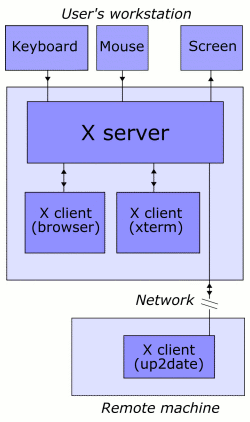
\includegraphics[width=.3\linewidth]{figures/X_client_server_example.png}
    \caption[xarch]{Esempio di architettura client-server di X Window System \footnotemark}
\end{figure}
\footnotetext{\emph{X client server example}: \url{https://commons.wikimedia.org/wiki/File:X_client_server_example.svg}}

La comunicazione tra server e client avviene in modalità full-duplex,
ovvero entrambi possono inviare e ricevere dati contemporaneamente.
%
Lo scambio di messaggi avviene tramite il protocollo TCP/IP,
ma spesso vengono utilizzati altri canali comunicativi come Unix domain sockets o memoria condivisa \footnote{\emph{The X New Developer’s Guide: Communication Between Client and Server}: \url{https://www.x.org/wiki/guide/communication/}}.
%
Indipendentemente dal canale utilizzato, è necessario che questo sia affidabile e che garantisca l'integrità e l'ordine dei messaggi,
in quanto il protocollo X non implementa nativamente meccanismi di ritrasmissione o di ordinamento dei pacchetti.
%
Quando un client si connette a un server X, avviene una fase di handshake che stabilisce la connessione e verifica l'autenticazione del client. Successivamente, il client può inviare richieste al server, come la creazione di finestre, il disegno di elementi grafici, o la gestione dell'input. Le richieste vengono accumulate in un buffer e inviate in modo asincrono per migliorare l'efficienza della comunicazione. Il server gestisce le richieste di più client contemporaneamente, garantendo l'isolamento tra loro, ma non fornisce alcuna garanzia di ordinamento tra client differenti, a meno che non venga esplicitamente richiesto \cite{xDevGuide}.

A differenza di altri protocolli progettati specificamente per il desktop remoto,
X è stato sviluppato principalmente per l'esecuzione remota di singole applicazioni grafiche,
piuttosto che per la gestione completa di un ambiente desktop (Desktop Environment, DE).
%
Per eseguire un intero DE in remoto, sarebbe necessario ricorrere a software aggiuntivi come X2Go.

Un'altra limitazione del protocollo X è l'assenza di meccanismi di compressione dei dati.
Questo significa che i dati grafici vengono trasmessi senza ottimizzazione,
il che può causare un utilizzo eccessivo della larghezza di banda e peggiorare le prestazioni su connessioni lente o instabili.
%
Inoltre, tutta la parte di rendering grafico è demandata alla macchina locale su richiesta del client.

\paragraph{Esempio di utilizzo di X Window System per l'esecuzione remota di applicazioni}

Per comprendere meglio il funzionamento del X Window System in un contesto di desktop remoto, consideriamo un esempio concreto:
l'esecuzione dell'applicazione di editing testuale \texttt{gedit} su un server remoto e la sua visualizzazione su un computer locale.
Questo può essere realizzato attraverso il X forwarding con ssh, utilizzando il seguente comando:

\begin{lstlisting}[caption={Connessione remota con X forwarding}, label={lst:ssh-x}, language=bash]
ssh -X user@remote_server
\end{lstlisting}

Dopo aver inserito le credenziali e stabilito la connessione, possiamo avviare l'applicazione da linea di comando come avremmo fatto localmente:

\begin{lstlisting}[caption={Esecuzione di gedit su server remoto}, label={lst:gedit}, language=bash]
gedit &
\end{lstlisting}

\paragraph{Funzionamento del protocollo}

Quando viene eseguito il codice di \Cref{lst:ssh-x},
il client e il server X avviano una procedura di handshake per stabilire il canale di comunicazione sicuro.
%
Il server X verifica che il client abbia i permessi necessari per connettersi al display locale e,
se tutto è corretto,
il client e il server negoziano parametri di comunicazione come il byte-ordering,
che permette di gestire correttamente i dati tra macchine con architetture diverse.

Dopo che l'handshake e la negoziazione dei parametri sono stati conclusi,
il client remoto \texttt{gedit} invia richieste al server X locale per creare finestre, disegnare interfacce grafiche e gestire l'input dell'utente.
%
Queste richieste vengono trasmesse attraverso il tunnel \texttt{ssh}.
%
Il client chiede inoltre al server X di intercettare gli eventi di input, come la pressione di un tasto o il movimento del mouse, e di inoltrarli al client remoto.
%
Quindi, quando l'utente interagisce con \texttt{gedit} (ad esempio digitando del testo o muovendo il mouse),
il server X cattura questi eventi e li inoltra al client remoto tramite il protocollo X11.
%
Il client elabora gli eventi e, se necessario, invia aggiornamenti grafici che vengono visualizzati sul display locale.
%
Questo flusso di comunicazione è gestito in modo asincrono, permettendo al server di accumulare richieste in un buffer e processarle in modo efficiente, ottimizzando così l'uso della rete.

\subsection{Virtual Network Computing}

Il protocollo \ac{VNC} è uno dei più diffusi per l'accesso remoto al desktop.
%
Sviluppato presso il laboratorio di ricerca Olivetti \& Oracle Research Laboratory nel 1998,
\ac{VNC} è stato inizialmente progettato per consentire l'accesso alle workstation da diversi dispositivi,
sia all'interno che all'esterno del laboratorio.
Sebbene X Window System offrisse già funzionalità simili, richiedeva che il dispositivo remoto eseguisse un server X,
che risultava spesso troppo oneroso per dispositivi con capacità di elaborazione limitate. Inoltre, X Window System era strettamente legato all'ambiente Unix \cite{richardson1998vnc}.

\ac{VNC}, al contrario, è stato concepito per essere indipendente dal sistema operativo e per garantire leggerezza nell'esecuzione.
Questo rende possibile la sua implementazione su qualsiasi dispositivo e l'accesso da qualunque altro dispositivo dotato di un client \ac{VNC},
anche poco potente.
%
Una delle caratteristiche chiave di \ac{VNC} è la semplicità del client, che non mantiene stati complessi,
permettendo una facile disconnessione e riconnessione senza compromettere lo stato del server o l'ambiente desktop.

\subsubsection{Architettura e funzionamento}

Alla base del sistema \ac{VNC} si trova il protocollo Remote Framebuffer (RFB)
\footnote{\textbf{\ac{VNC}} - \emph{Wikipedia}: \url{https://w.wiki/BoHJ}},
che opera a livello di framebuffer,
rendendolo compatibile con qualsiasi sistema operativo,
sistema di finestre o applicazione.
%
Il sistema \ac{VNC} è composto principalmente da due componenti:
il server \ac{VNC} e il client \ac{VNC}.
%
Il server è responsabile delle modifiche al framebuffer e ospita il sistema di finestre e le applicazioni,
mentre il client rappresenta l'endpoint con cui l'utente interagisce attraverso il display e i dispositivi di input \cite{richardson1998vnc}.

\paragraph{Rendering grafico}

Il sistema \ac{VNC} utilizza un metodo di rendering molto semplice, basato su una singola operazione grafica:
\begin{quote}
    "Posiziona un rettangolo di dati di pixel in una determinata posizione \emph{x}, \emph{y}."
\end{quote}
Questo approccio, pur sembrando inefficiente a prima vista, offre grande flessibilità grazie all'uso di diversi schemi di codifica dei dati grafici.
%
Ad esempio il server può ottimizzare la trasmissione di dati riciclando informazioni già presenti sullo schermo del client.
%
Se una finestra viene spostata da una posizione all'altra sul desktop,
il server \ac{VNC} invierà semplicemente una richiesta per spostare il rettangolo corrispondente dalla posizione iniziale (\texttt{x1, y1}) alla nuova posizione (\texttt{x2, y2}).
%
Inoltre, \ac{VNC} utilizza tecniche di compressione dei dati per ridurre significativamente la quantità di informazioni da trasmettere.

Un insieme di rettangoli di pixel modificati viene definito "framebuffer update".
Ogni rettangolo può essere codificato in modo diverso,
consentendo al server di scegliere il metodo di codifica più efficiente in base alla situazione.
%
A differenza di un frame video completo,
un aggiornamento del framebuffer riguarda solo la porzione di schermo modificata.
%
Gli aggiornamenti vengono inviati in modo asincrono: il server invia nuovi aggiornamenti solo quando è necessario;
questo consente di adattare la frequenza degli aggiornamenti in base agli eventi sullo schermo, alla velocità della rete e alle capacità del client \cite{richardson1998vnc}.
%
Ad esempio, se l'utente trascina una finestra su una connessione veloce con un client potente,
gli aggiornamenti saranno continui e fluidi. In caso di connessione lenta o client con risorse limitate,
il server ridurrà la frequenza degli aggiornamenti, causando un movimento meno fluido.

\paragraph{Input}

\ac{VNC} supporta un modello standard di input che include una tastiera e un dispositivo di puntamento multi-pulsante.
Il client invia eventi di input ogni volta che un tasto viene premuto o il mouse viene mosso, permettendo al server di elaborare questi eventi e aggiornare l'interfaccia di conseguenza. \cite{richardson1998vnc}.

\paragraph{Connessione e autenticazione}

Quando un client richiede la connessione a un server \ac{VNC},
il server risponde con una richiesta di autenticazione,
generalmente basata su un meccanismo di password \textit{challenge-response}.
%
Una volta autenticato, client e server negoziano parametri come la risoluzione dello schermo,
il formato dei pixel, i metodi di codifica supportati e altre impostazioni.
%
Dopo la negoziazione, la sessione viene avviata e il client richiede il primo aggiornamento del framebuffer \cite{richardson1998vnc}.

\subsection{Remote Desktop Protocol}

\ac{RDP} è un protocollo proprietario sviluppato da Microsoft per l'accesso remoto a sistemi Windows.
Viene introdotto nel 1998 con Windows NT 4.0 Terminal Server Edition e successivamente integrato in tutte le versioni successive di Windows (ad eccezione delle versioni Home).

\subsubsection{Il Protocollo}
Al suo interno lo stack \ac{RDP} è composto da diversi protocolli, ognuno con un compito specifico.
\begin{itemize}
    \item \textbf{TPKT}: Anche conosciuto come \emph{ISO Transport Service on top of the TCP (RFC 1006)}, è un protocollo di trasporto che fornisce un servizio di trasporto orientato alla connessione
     Permette lo scambio di unità di dati \ac{TPDU} tra due host.
    \item \textbf{X.224}: Protocollo di livello di trasporto che fornisce servizi di sessione e di connessione. Gestisce le richieste e risposte di connessione.
    \item \textbf{T.125 MCS}: Protocollo che permette ad \ac{RDP} di gestire e comunicare attraverso più canali di comunicazione.
\end{itemize}

L'attività di invio e ricezione dei dati tramite lo stack \ac{RDP} segue essenzialmente lo stesso schema del modello OSI a sette livelli,
comune nelle reti \ac{LAN}.
%
I dati di un'applicazione o servizio vengono segmentati,
indirizzati a un canale, crittografati,
incapsulati e impacchettati nel protocollo di rete, per poi essere inviati al client.
%
I dati ricevuti subiscono il processo inverso: vengono decapsulati, decrittografati e, infine, resi disponibili all'applicazione. \cite{microsoftrdp}

\subsubsection{Connessione}

La fase di connessione può essere suddivisa nelle seguenti fasi:
\begin{enumerate}
    \item \textbf{Inizializazione della connessione}: Il client invia un \ac{PDU} di richiesta di connessione utilizzando il protocollo X.224. Il server risponde con un \ac{PDU} di conferm di connessione.
    In questa fase viene stabilito il protocollo di sicurezza da utilizzare.
    \item \textbf{Scambio delle Impostazioni di Base}: Tramite MCS Connect Initial \ac{PDU} e MCS Connect Response \ac{PDU},
    client e server scambiano informazioni di base come la versione del protocollo, la dimesione del desktop,
    dati riguardanti la sicurezza come il server random e il certificato e informazioni di rete come il numero di canali supportati.
    \item \textbf{Connessione dei Canali}: Il client e il server stabiliscono le connessioni individuali per ogni canale virtuale previsto nella sessione,
    tramite una serie di richieste e conferme.
    \item \textbf{Avvio della Sicurezza}: Il client invia un \ac{PDU} di scambio di sicurezza contenente un numero casuale cifrato, utile per generare le chiavi di sessione.
    Da questo punto, il traffico \ac{RDP} può essere cifrato.
    \item \textbf{Scambio delle Impostazioni di Sicurezza}: Il client invia un \ac{PDU} criptato contenente informazioni di configurazione come username,
    dominio e opzioni di compressione supportate.
    \item \textbf{Verifica della Licenza}: Questa fase verifica se il client è autorizzato a connettersi a un terminal server con un numero maggiore di connessioni simultanee.
    Se il server non ha una licenza configurata, consente fino a due connessioni.
    \item \textbf{Scambio delle Funzionalità supportate}: Il server e il client scambiano informazioni sui rispettivi tipi di capacità supportati, come codec per bitmap,
    supporto per tastiera e mouse, e configurazioni generali.
    \item \textbf{Finalizzazione della Connessione}: Il client e il server completano la connessione attraverso una serie di \ac{PDU}s per sincronizzare i rispettivi identificatori utente e definire il controllo condiviso della sessione.
    \item \textbf{Scambio dei Dati}: Una volta stabilita la connessione, il client invia dati di input (come tastiera e mouse) e riceve output grafico dal server,
    con l’opzione di utilizzare la compressione per ridurre il traffico dati.
\end{enumerate}

\subsubsection{Input e Output}
Durante una sessione \ac{RDP}, il client invia dati di input (come ad esempio mouse e tastiera) al server, mentre quest'ultimo invia al client dati di output, principalmente grafici.
Questo scambio di dati avviene attraverso due modalità: \textit{slow-path} e \textit{fast-path}:
\begin{itemize}
    \item \textbf{Slow-Path}: Questa modalità è la più completa, in cui ogni pacchetto di dati \ac{PDU} include l'intera serie di header del protocollo \ac{RDP}.
    Questo lo rende adatto per inviare dati critici che richiedono la piena gestione dei metadati, anche se aumenta la dimensione dei pacchetti trasmessi e il consumo di banda.
    \item \textbf{Fast-Path}: Riducendo o rimuovendo alcuni degli header da alcuni \ac{PDU},
    questa modalità permette di ridurre la quantità di dati trasmessi e la latenza di trasmissione.
    Inoltre così facendo riduce anche il carico di lavoro per processare i pacchetti.
    Fast-Path è comunemente usato per input a bassa priorità, come movimenti del mouse e sequenze di tasti, dove è importante minimizzare il ritardo.
\end{itemize}

\subsubsection{Canali in RDP}
\ac{RDP} si avvale di diversi canali per la trasmissione di dati. Esistono due tipi principali di canali:
\begin{itemize}
    \item \textbf{\ac{SVC}}: Limitati a 31 per connessione,
    questi canali trasportano comunicazioni essenziali tra client e server, come il canale I/O o il canale utente. Vengono instaurati durante lo "Scambio delle Impostazioni di Base" e rimangono attivi per tutta la durata della sessione.
    \item \textbf{\ac{DCV}}: Trasportati su uno specifico \ac{SVC} (chiamato \emph{DRDYNVC}),
    i \ac{DCV}, a differenza degli \ac{SVC},
    possono essere creati e distrutti liberamente durante la sessione.
    Questi canali possono essere liberamente utilizzate da sviluppatori per estendere le funzionalità di \ac{RDP}.
    Utilizzi comuni sono l'input audio (da client a server), rendering grafico e PnP.
\end{itemize}

\subsection{Parsec}
Parsec è un software di desktop remoto focalizzato principalmente sul gaming. Rispetto alle tecnologie precedenti è ideato per ridurre al minimo la latenza tra il client e il server.
La capacità di offrire streaming video a bassa latenza, alta risoluzione e alto frame rate lo rende adatto non solo per il gaming ma anche per applicazioni professionali come l'editing video o la progettazione grafica.
Nasce dall'idea di utilizzare istanze GPU di Amazon Web Services per lo streaming di giochi a bassa latenza su dispositivi meno potenti e successivamente si evolve in un servizio di desktop remoto completo.
%
A differenza di alcune tecnologie sopra citate,
Parsec trasmette come flusso video un "mirror" del desktop dove è presente il server,
permettendo di visualizzare l'intero ambiente desktop e non solo singole applicazioni. Quindi parsec si comporta come se dovesse trasmettere un video.
Aggiungendo la possibilità di trasmettere input da tastiera e mouse, il client può interagire con il server come se si trovasse fisicamente davanti ad esso.

Il client Parsec è disponibile per Windows, macOS, Linux, Android, Raspberry Pi e web browser. Il server Parsec è disponibile per Windows e macOS. 

\subsubsection{Procedura di Trasmissione e Visualizzazione}

Il flusso di lavoro di Parsec per la trasmissione video si compone delle seguenti fasi:
\begin{enumerate}
    \item Cattura del frame
    \item Compressione
    \item Trasmissione
    \item Decodifica
    \item Rendering
\end{enumerate}

\paragraph{Cattura del frame}
Per la cattura del frame su Windows, Parsec utilizza la Desktop Duplication API (disponibile a partire da Windows 8.1),
che consente diretto accesso al framebuffer e permette di trasferire il frame nella memoria video della GPU.

\paragraph{Compressione}
Per poter trasmettere questo flusso video ad alta risoluzione e frame rate su una rete, è necessario comprimerlo.
La compressione di un video può essere eseguita in due modi: software e hardware.
%
La compressione software è eseguita dalla CPU, mentre la compressione hardware è eseguita da un chip dedicato, come una GPU (integrata o dedicata).
%
Il vantaggio della compressione software è la compatibilità in quanto può essere eseguita su qualsiasi dispositivo, ma il suo svantaggio è il tempo impiegato per la compressione.
La compressione hardware, al contrario, è molto più veloce ma richiede un chip dedicato, che non è sempre presente su tutti i dispositivi.
%
Parsec utilizza i codec H.264 e H.265, scelti per la loro ampia compatibilità hardware così da permettere compressione hardware per qualsiasi dispositivo relativamente recente.

Per ridurre al minimo le latenza, Parsec è progettato per far si che il framebuffer,
una volta catturato, venga direttamente inviato alla GPU per essere codificato senza passare per la memoria di sistema, evitando operazioni CPU intermedie.

\paragraph{Trasmissione}
Per garantire una connessione a bassa latenza, Parsec utilizza due connessione Peer-To-Peer UDP sia per client che per host.

\paragraph{Decodifica}
Una volta ricevuto dal client, il frame compresso viene decodificato. Anche in questo caso Parsec predilige la decodifica hardware, sfruttando ASIC o GPU per ridurre al minimo la latenza.

\paragraph{Rendering}
L'ultimo passaggio della procedura è il rendering, che consiste nel visualizzare il frame decodificato sullo schermo del client. Parsec, per minimizzare i ritardi e garantire una visione fluida, utilizza la sincronizzazione verticale (V-sync) per allineare la visualizzazione del frame con il refresh rate del monitor, evitando problemi di tearing. Questo implica una sincronizzazione accurata tra i frame inviati dal server e il display del client.

\subsubsection{Latenza}
Come abbiamo detto, la sfida principale di Parsec è ridurre al minimo la latenza tra il client e il server. Eseguendo tutte le operazioni sulla GPU, evitando che la CPU sia coinvolta nella compressione e decompressione dei frame, Parsec riesce a ridurre la latenza a pochi millisecondi. Inoltre, utilizzando connessioni Peer-To-Peer UDP, Parsec evita i ritardi dovuti ai server intermedi, garantendo una connessione diretta tra client e host. Una limitazione che Parsec non può superare è la latenza intrinseca della rete, che può variare in base alla qualità della connessione e alla distanza geografica tra client e server. Fortunatamente negli ultimi anni la diffusione di connessioni ad alta velocità e a bassa latenza è aumentata notevolmente, sopratutto con l'aumento di connessioni Fiber To The Home (FTTH).

\subsubsection{Altri Utilizzi}
Grazie alla sua capacità di trasmettere video ad alta risoluzione e frame rate, Parsec è spesso utilizzato non solo per cloud gaming o desktop remoto Over The Internet, ma anche per Local Game Streaming. Questo consiste nell'avere una macchina potente da cui potersi collegare da altri dispositivi meno potenti, come una smart TV, così da poter avere un'esperienza di gioco di alta qualità su un dispositivo che altrimenti non sarebbe in grado di supportare i giochi più recenti.

\subsection{Menzioni d'onore}
Ci sono altri protocolli proprietari che meritano una menzione, come lo storico Team-Viewer o AnyDesk, che offrono funzionalità di desktop remoto per utenti meno esperti grazie ad un setup minimo evitando l'apertura di porte. Purtroppo le informazioni sul funzionamento di questi sono molto limitate e non è possibile approfondire ulteriormente.

\paragraph{Moonlight e Sunshine}
NVIDIA, con la tecnologia Gamestream, permetteva di trasmettere il flusso video di un gioco da un computer con una GPU NVIDIA ad un dispositivo NVIDIA Shield. Per poter utilizzare questa funzione, e il server messo a disposizione dai driver NVIDIA, e ricevere questo flusso su ogni dispositivo, la community open-source ha sviluppato Moonlight, un client compatibile con qualsiasi dispositivo Android, iOS, Windows, macOS e Linux, in grado di ricevere il flusso video da un server NVIDIA Gamestream.

Quando nel 2022 NVIDIA ha deciso di rimuovere il supporto per i server Gamestream, la community ha sviluppato Sunshine, un server open-source in grado di trasmettere il flusso video di un gioco da un computer con una qualsiasi GPU (Gamestream era limitato a NVIDIA) ad un client Moonlight.
Con il passare del tempo Sunshine è migliorato notevolmente, ed utilizzando un concetto molto simile a quello di Parsec, è in grado di ottenere latenze molto basse, rendendolo adatto non solo per il gaming, ma anche per applicazioni professionali. Inoltre la sua natura open-source e i continui impegni della community a migliorarlo, lo rendono migliore di molte soluzioni proprietarie. Sunshine infatti, rispetto a Parsec, è disponibile anche su Linux, oltre che su Windows e macOS. Supporta inoltre numerosi metodi di cattura e permette all'utente di modificare parametri come la qualità del video, la risoluzione e il frame rate, in base alle necessità e alla potenza del computer.

\chapter{Sviluppi e Applicazioni Attuali delle Tecnologie di Desktop Remoto}
\label{chap:current-applications}
% -- VDI, Cloud Gaming, Smart working, Assistenza Remota, DaaS, Applicazioni virtualizzate

In questo capitolo verranno analizzati gli sviluppi e le applicazioni delle tecnologie di desktop remoto attualmente in uso. Negli ultimi anni, l'utilizzo delle soluzioni di accesso remoto si è ampliato, adattandosi alle esigenze di settori diversi, dai contesti lavorativi tradizionali a settori emergenti come il cloud gaming e le piattaforme di collaborazione virtuale. Le tecnologie moderne hanno raggiunto livelli di prestazioni e sicurezza avanzati, rendendo il desktop remoto un elemento centrale nel telelavoro, nell'assistenza tecnica e nelle applicazioni di streaming in tempo reale.

Di seguito si esamineranno le principali applicazioni delle tecnologie di desktop remoto oggi disponibili, con particolare attenzione all’ottimizzazione delle risorse di rete, alla sicurezza e alle modalità d'uso nei vari contesti.

\section{Infrastructure as a Service (IaaS)}
\label{sec:iaas}
Un possibile e diffuso utilizzo delle tecnologie di desktop remoto è il suo impiego all'interno di servizi di cloud computing, in particolare nell'ambito dell'Infrastructure as a Service (IaaS).
Infrastructure as a Service è un termine che indica un modello di servizio dove un fornitore di servizi cloud mette a disposizione degli utenti risorse hardware virtualizzate, come server, reti, spazio di archiviazione e sistemi operativi, su richiesta. In poche parole permette all'utente di noleggiare un'infrastruttura IT completa, senza dover acquistare o gestire fisicamente hardware e strutture di rete \cite{bhardwaj2010cloud}.

\subsection{Caratteristiche di IaaS}
Un provide di servizi IaaS mette a disposizione dell'utente l'hardware (tipicamente virtualizzato), i servizi amministrativi per la gestione delle risorse e una piattaforma per poter eseguire applicativi (come sistemi operativi).
Come ogni servizio di cloud computing, IaaS ricade sotto queste cinque caratteristiche fondamentali:
\begin{itemize}
    \item \textbf{Self-service on demand}: l'utente può richiedere e configurare risorse in modo autonomo, senza l'intervento del fornitore;
    \item \textbf{Ampio accesso alla rete}: le risorse sono accessibili tramite Internet o una rete privata;
    \item \textbf{Risorse condivise}: le risorse sono condivise tra più utenti, garantendo efficienza e scalabilità;
    \item \textbf{Risorse scalabili}: le risorse possono essere allocate e deallocate rapidamente in base alle esigenze;
    \item \textbf{Misurabilità del servizio}: l'uso delle risorse può essere monitorato e misurato, consentendo una gestione efficiente dei costi.
\end{itemize}
Questo porta a una serie di vantaggi per le aziende o gli utenti che ne fanno uso, tra cui:
\begin{itemize}
    \item \textbf{Costo incrementale}: l'utente paga solo per le risorse effettivamente utilizzate e per il tempo di utilizzo;
    \item \textbf{Ampio storage}: possibilità di archiviare grandi quantità di dati in modo scalabile;
    \item \textbf{Mantenimento semplificato}: il fornitore si occupa della manutenzione dell'hardware e degli aggiornamenti software (almeno quelli di base);
    \item \textbf{Accesso globale}: le risorse sono accessibili da qualsiasi luogo connesso a Internet;
    \item \textbf{Flessibilità e scalabilità}: le risorse possono essere adattate alle esigenze specifiche dell'applicazione e aumentate o ridotte rapidamente;
\end{itemize}   
Per questo ed altri motivi, l'IaaS è diventato uno dei modelli di servizio più diffusi nel cloud computing. Affiancato ad una tecnologia di Desktop Remoto a bassa latenza, permette di avere un'esperienza di utilizzo indistinguibile da un computer fisico, con la flessibilità e la scalabilità tipiche del cloud computing.

\subsection{Provider e Cliente}
\label{subsec:provider_cliente}

Nel modello Infrastructure as a Service (IaaS), il \textbf{Provider} e il \textbf{Cliente} svolgono ruoli distinti e complementari. Il Provider è responsabile della gestione dell'infrastruttura fisica e virtuale, come server, rete e sistemi di archiviazione, garantendo sicurezza e continuità del servizio. Inoltre, il Provider si occupa del monitoraggio continuo delle risorse, della manutenzione e degli aggiornamenti, così come della scalabilità, permettendo al Cliente di aumentare o ridurre le risorse in base alle proprie necessità. Il livello di servizio viene formalizzato in specifici SLA (Service Level Agreements), che stabiliscono standard di disponibilità e prestazioni.

Dall'altra parte, il Cliente gestisce le proprie applicazioni e dati all'interno dell'infrastruttura fornita. Pur non essendo coinvolto nella gestione dell'hardware, il Cliente è responsabile della configurazione del software, della protezione dei dati e dell'accesso sicuro alle applicazioni. Inoltre, deve monitorare l'uso delle risorse per ottimizzare i costi e garantire la conformità alle normative di settore.

In questo modello, Provider e Cliente lavorano in sinergia per garantire un uso efficiente e sicuro delle risorse cloud: il Provider fornisce la piattaforma infrastrutturale e ne assicura il funzionamento, mentre il Cliente ne sfrutta le potenzialità per eseguire le proprie applicazioni e gestire i propri dati.



\chapter{Prospettive, Sviluppi e Applicazioni futuri del Desktop Remoto}
% -- IA upscaling per ridurre latenza, Edge Computing, Fog Computing, AR VR, Blockchain?

\section{Edge Computing}

\section{...}

\chapter{Conclusioni}
\label{chap:conclusions}

%----------------------------------------------------------------------------------------
% BIBLIOGRAPHY
%----------------------------------------------------------------------------------------

\backmatter

\nocite{*} % Remove this as soon as you have the first citation

\bibliographystyle{acm}
\bibliography{bibliography}    

\begin{acknowledgements} % this is optional
Optional. Max 1 page.
\end{acknowledgements}

\end{document}
